% Created 2026-04-22 Wed 22:22
% Intended LaTeX compiler: lualatex
\DocumentMetadata{lang = en, pdfversion = 2.0, pdfstandard = ua-2, pdfstandard = a-4, testphase = {phase-III, title, table, math, firstaid}}
\documentclass[11pt]{article}
\usepackage{amsmath}
\usepackage{fontspec}
\usepackage{graphicx}
\usepackage{longtable}
\usepackage{wrapfig}
\usepackage{rotating}
\usepackage[normalem]{ulem}
\usepackage{capt-of}
\usepackage{hyperref}
\usepackage[margin=1in]{geometry}
\usepackage{fontspec}
\usepackage{verbatim, multicol, tabularx,}
\usepackage{amsmath, amsthm, amssymb, stmaryrd, latexsym, bm, listings, qtree}
\usepackage{framed}
\usepackage{xcolor,colortbl}
\usepackage{media9}
\usepackage[export]{adjustbox}
\usepackage{algorithm}
\usepackage[noend]{algpseudocode}
\usepackage{tikz,pgfplots}
\usetikzlibrary{shapes.geometric}
\let\oldquote=\quote
\let\endoldquote=\endquote
\colorlet{shadecolor}{cyan!15}
\renewenvironment{quote}{\begin{shaded*}\begin{oldquote}}{\end{oldquote}\end{shaded*}}
% From https://tex.stackexchange.com/questions/7032/good-way-to-make-textcircled-numbers
\newcommand*\circled[1]{\tikz[baseline=(char.base)]{\node[shape=circle,draw,inner sep=2pt] (char) {#1};}}
\DeclareMathOperator*{\argmin}{arg\!min}
\DeclareMathOperator*{\argmax}{arg\!max}
\lstset{frame=tb, aboveskip=1mm, belowskip=0mm, showstringspaces=false, columns=flexible, basicstyle={\scriptsize\ttfamily}, numbers=left, frame=single, breaklines=true, breakatwhitespace=true}
\hypersetup{colorlinks=true,urlcolor=blue}
\usepackage{polyglossia}
\setdefaultlanguage[variant=US]{english}
\author{Christopher Simpkins}
\date{Kennesaw State University}
\title{Artificial Intelligence\\\medskip
\large Adversarial Search}
\hypersetup{
 pdfauthor={Christopher Simpkins},
 pdftitle={Artificial Intelligence},
 pdfkeywords={},
 pdfsubject={Artificial Intelligence Adversarial Search},
 pdfcreator={Emacs 30.2 (Org mode 9.7.11)}, 
 pdflang={English}}
\begin{document}

\maketitle
\section{Games}
\label{sec:orgbe9f6ec}

\textbf{Competitive environments}, in which two or more agents have conflicting goals, give rise to \textbf{adversarial search} problems.

Three approaches to dealing with multiagent environments:

\begin{enumerate}
\item With a large number of agents, consider aggregates of agents as an \textbf{economy}, e.g., supply-demand relationships, without predicting actions of any individual agents.

\item Consider adversarial agents as just a part of the environment—a part that makes the environment nondeterministic. But if we model the adversaries in the same way that, say, rain sometimes falls and sometimes doesn’t, we miss the idea that our adver- saries are actively trying to defeat us, whereas the rain supposedly has no such intention.

\item Explicitly model the adversarial agents with the techniques of adversarial game-tree search.
\end{enumerate}

This lesson deals with the third approach.
\section{From Game Theory to Adversarial AI}
\label{sec:org9ab10d0}

In game theory, games like Chess and Go are deterministic, two-player, turn-taking, perfect information, zero-sum games.

\begin{center}
\begin{tabular}{ll}
Game Theory & AI\\
\hline
Perfect information & Fully observable\\
Player & Agent\\
Move & Action\\
Position & State\\
Payoff/Score & Utility/Reward/Value\\
\end{tabular}
\end{center}

In AI we commonly study two-player zero sum games, in which the "score" for one agent is the negative of the other agent's, i.e., they add to zero.

\begin{quote}
Note: in Chess tournaments draws award each player scores of \(\frac{1}{2}\), but in an AI chess playing algorithms you can use +1, -1, and 0.  Alternatively, you can model chess as a "constant sum" game with scores of 1, 0, or \(\frac{1}{2}\).
\end{quote}
\section{Two-Player Zero-Sum Games}
\label{sec:org44a18b7}

Two players: MAX and MIN.  MAX moves first.

A game can be formally defined with the following elements:

\begin{itemize}
\item \(S_0\): The initial state, which specifies how the game is set up at the start.

\item \(ToMove(s)\): The player whose turn it is to move in state \(s\), MAX or MIN.

\item \(Actions(s)\): The set of legal moves in state \(s\).

\item \(Result(s, a)\): The transition model, which defines the state resulting from taking action \(a\) in state \(s\).

\item \(IsTerminal(s)\): A terminal test, which is true when the game is over and false otherwise. States where the game has ended are called terminal states.

\item \(Utility(s,p)\): A utility function (also called an objective function or payoff function), which defines the final numeric value to player \(p\) when the game ends in terminal state \(s\).  In chess, the outcome is a win, loss, or draw, with values 1, 0, or 1/2. Some games have a wider range of possible outcomes—for example, the payoffs in backgammon range from 0 to 192.
\end{itemize}
\section{Tic-Tac-Toe Game Tree}
\label{sec:org08b67e9}


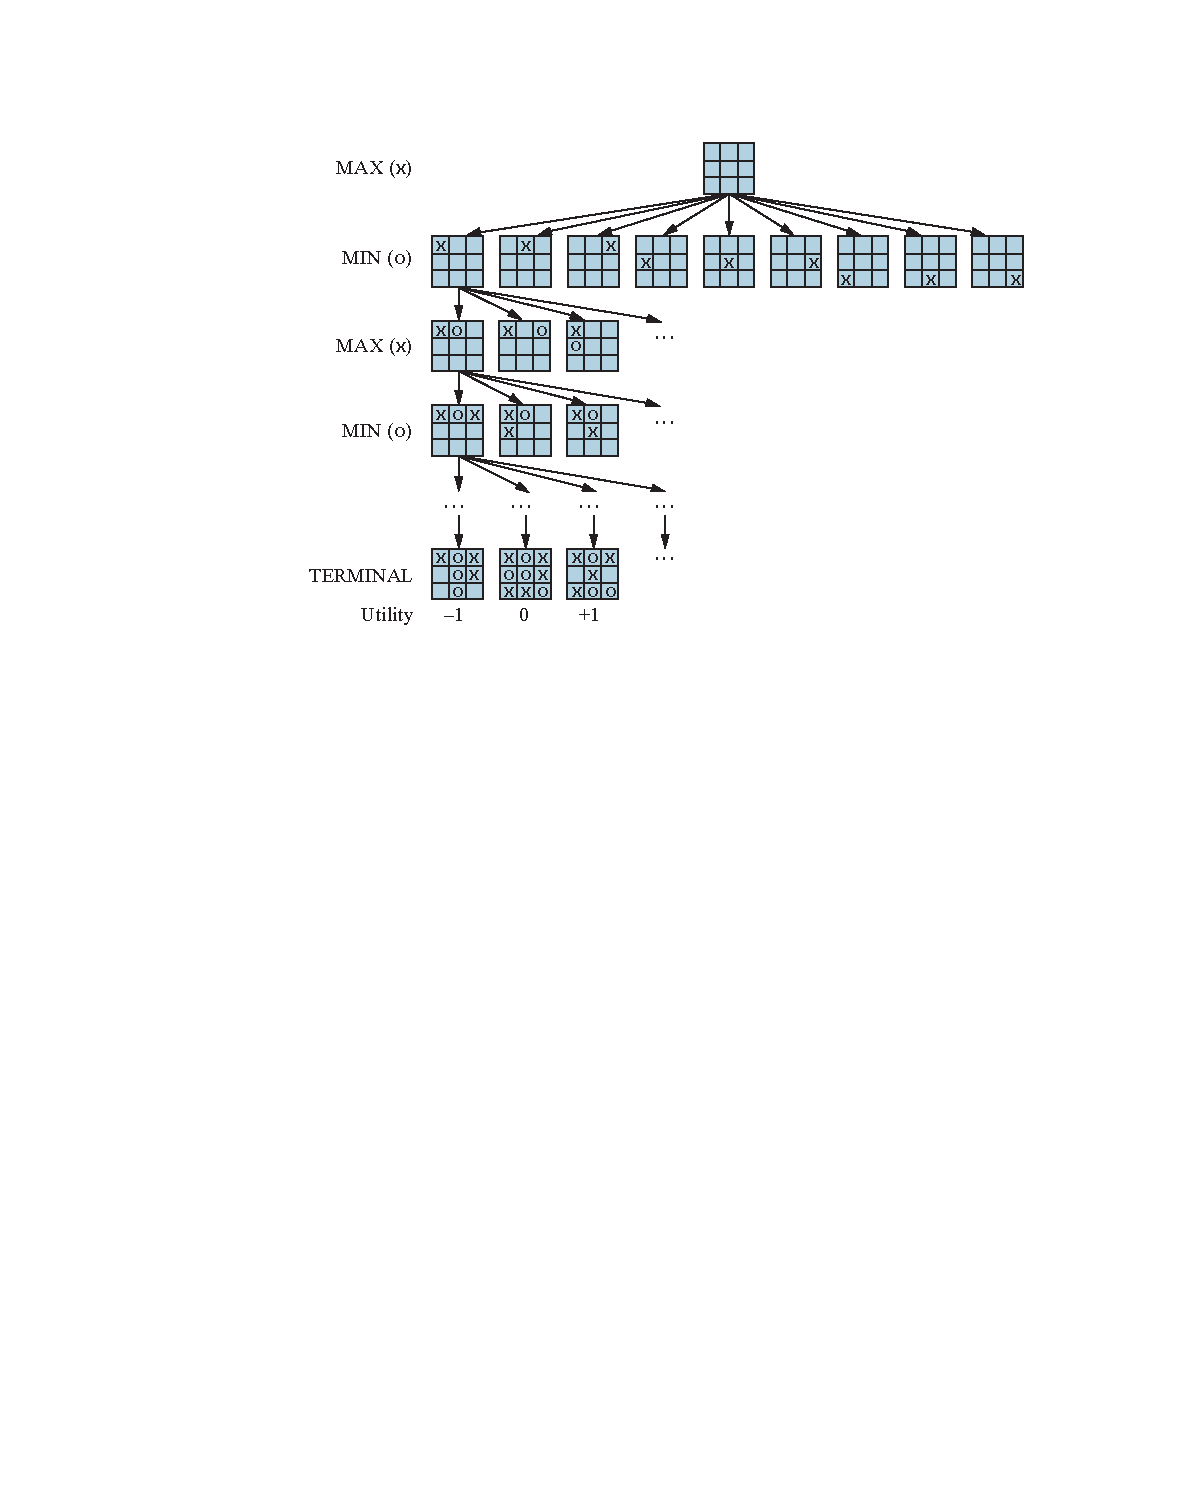
\includegraphics[alt={aima fig 05_01 tic tac toe game tree},height=2.8in]{aima-fig-05_01-tic-tac-toe-game-tree.pdf}



Tic-tac-toe is relatively small -- fewer than \(9!= 362,880\) terminal nodes with only 5,478 distinct states.
\section{Optimal Decisions in Games}
\label{sec:org2342443}

\begin{itemize}
\item MAX searches for a sequence of actions leading to a win.
\item MIN searches for a sequence of actions leading to a loss for MAX.
\item So MAX's stratregy is a contingfency plan dependent on MIN's responses.
\item We could use AND-OR search, but we'll study a more general approach: \textbf{minimax search}.
\end{itemize}

Minimax search generates a game tree with moves for both MAX and MIN

\begin{itemize}
\item At each MAX node, choose from actions \(a \in Actions(s)\) with maximum value relative to MAX.
\item At each MIN node, choose from actions \(b \in Actions(s)\) with minimum value relative to MAX.
\item One move by one player is called a \textbf{ply}.  A ply for MAX plus the response ply for MIN constitute a game move.
\end{itemize}
\section{Minimax Decision}
\label{sec:org622a7d8}

\begin{itemize}
\item Given a game tree, the optimal strategy can be determined by working out the \textbf{minimax value} of each state in the tree, which we write as \(Minimax(s)\).

\item The minimax value is the utility (for MAX) of being in that state, assuming that both players play optimally from there to the end of the game. The minimax value of a terminal state is just its utility.
\end{itemize}

\begin{equation*}
Minimax(s) =
\begin{cases}
Utility(s,MAX)                              & \text{if } IsTerminal(s) \\
max_{a \in Actions(s)} Minimax(Result(s,a)) & \text{if } ToMove(s) = MAX \\
min_{a \in Actions(s)} Minimax(Result(s,a)) & \text{if } ToMove(s) = MIN
\end{cases}
\end{equation*}
\section{Minimax Game Tree}
\label{sec:orgda48ed4}


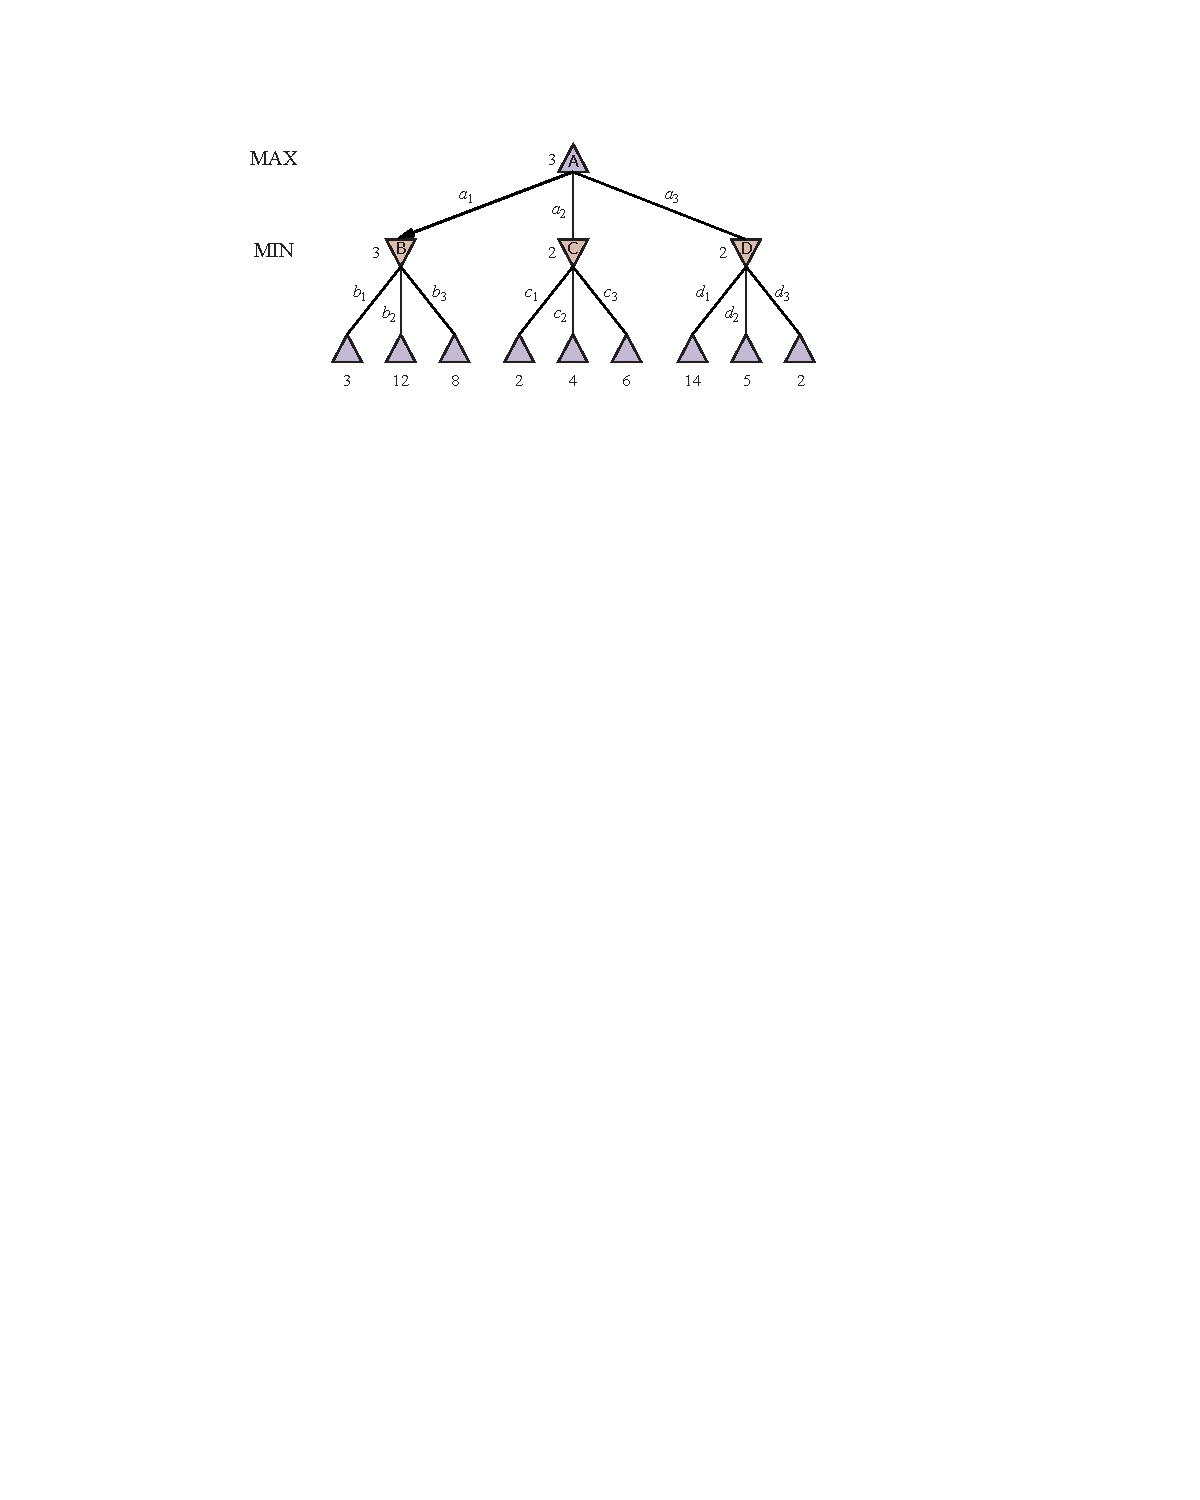
\includegraphics[alt={aima fig 05_02 two ply game tree},width=0.75\linewidth]{aima-fig-05_02-two-ply-game-tree.pdf}



A two-ply game tree.

\begin{itemize}
\item \(\triangle\) nodes are "MAX nodes," --  MAX’s turn to move.
\item \(\triangledown\) nodes are "MIN nodes."
\item Terminal nodes show the utility values for MAX.
\item Other nodes are labeled with their minimax values.
\item MAX’s best move at the root is \(a_1\), because it leads to state with highest minimax value.
\item MIN’s best reply is \(b_1\), because it leads to the state with the lowest minimax value.
\end{itemize}
\section{Minimax Algorithm}
\label{sec:org5ffd017}




\begin{itemize}
\item Recurse through MIN and MAX plies of the game tree to leaf nodes.
\item Back up minimax values through the tree.
\item Choose branch with highest minimax value.
\end{itemize}





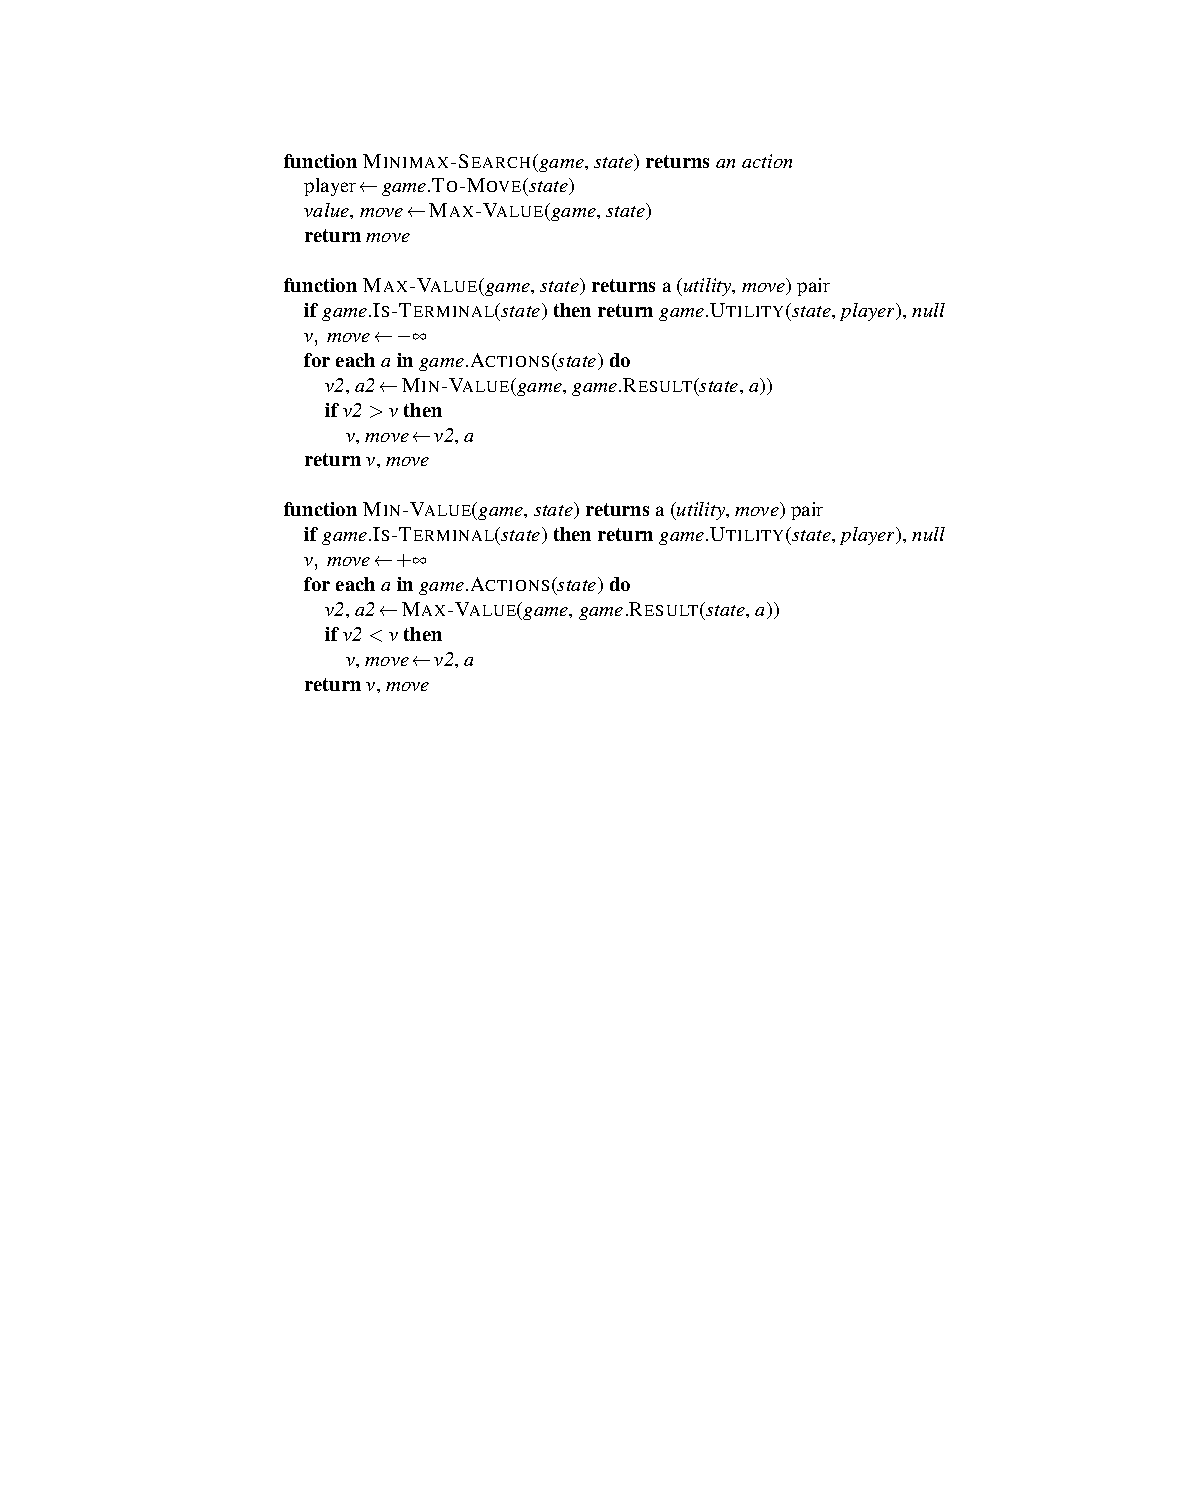
\includegraphics[alt={aima fig 05_03 minimax algorithm},width=0.75\linewidth]{aima-fig-05_03-minimax-algorithm.pdf}
\section{Analysis of Minimax}
\label{sec:org6944818}

\begin{itemize}
\item Time complexity: \(O(b^m)\)
\item Space complexity:

\begin{itemize}
\item \(O(bm)\) if generates all actions at once
\item \(O(m)\) if generates actions one at a time
\end{itemize}
\end{itemize}

Chess has an average branching factor of 35 and an average game has a depth of 80.

\begin{itemize}
\item \(O(b^m) = 35^{80} \approx 10^{123}\) states
\end{itemize}

Clearly, minimax won't work for Chess.  We'll make two modifications to minimax that makes games like Chess tractable.
\section{Alpha-Beta Pruning}
\label{sec:orgbb8b8ec}

Number of game states is exponential in depth of tree, so we have to \textbf{prune} branches of the tree to make searching it tractable.


\begin{itemize}
\item \(\alpha\) = the value of the best (i.e., highest-value) choice we have found so far at any choice point along the path for MAX.

\begin{itemize}
\item Think: \(\alpha\) = "at least."
\end{itemize}

\item \(\beta\) = the value of the best (i.e., lowest-value) choice we have found so far at any choice point along the path for MIN.

\begin{itemize}
\item Think: \(\beta\) = "at most."
\end{itemize}
\end{itemize}

Alpha-beta pruning cuts off the exploration of nodes if those nodes would not change move selection.
\section{Alpha-Beta Pruning in Action}
\label{sec:org4d84f93}

Intervals show range of possible values at each node,  \([\alpha, \beta]\).


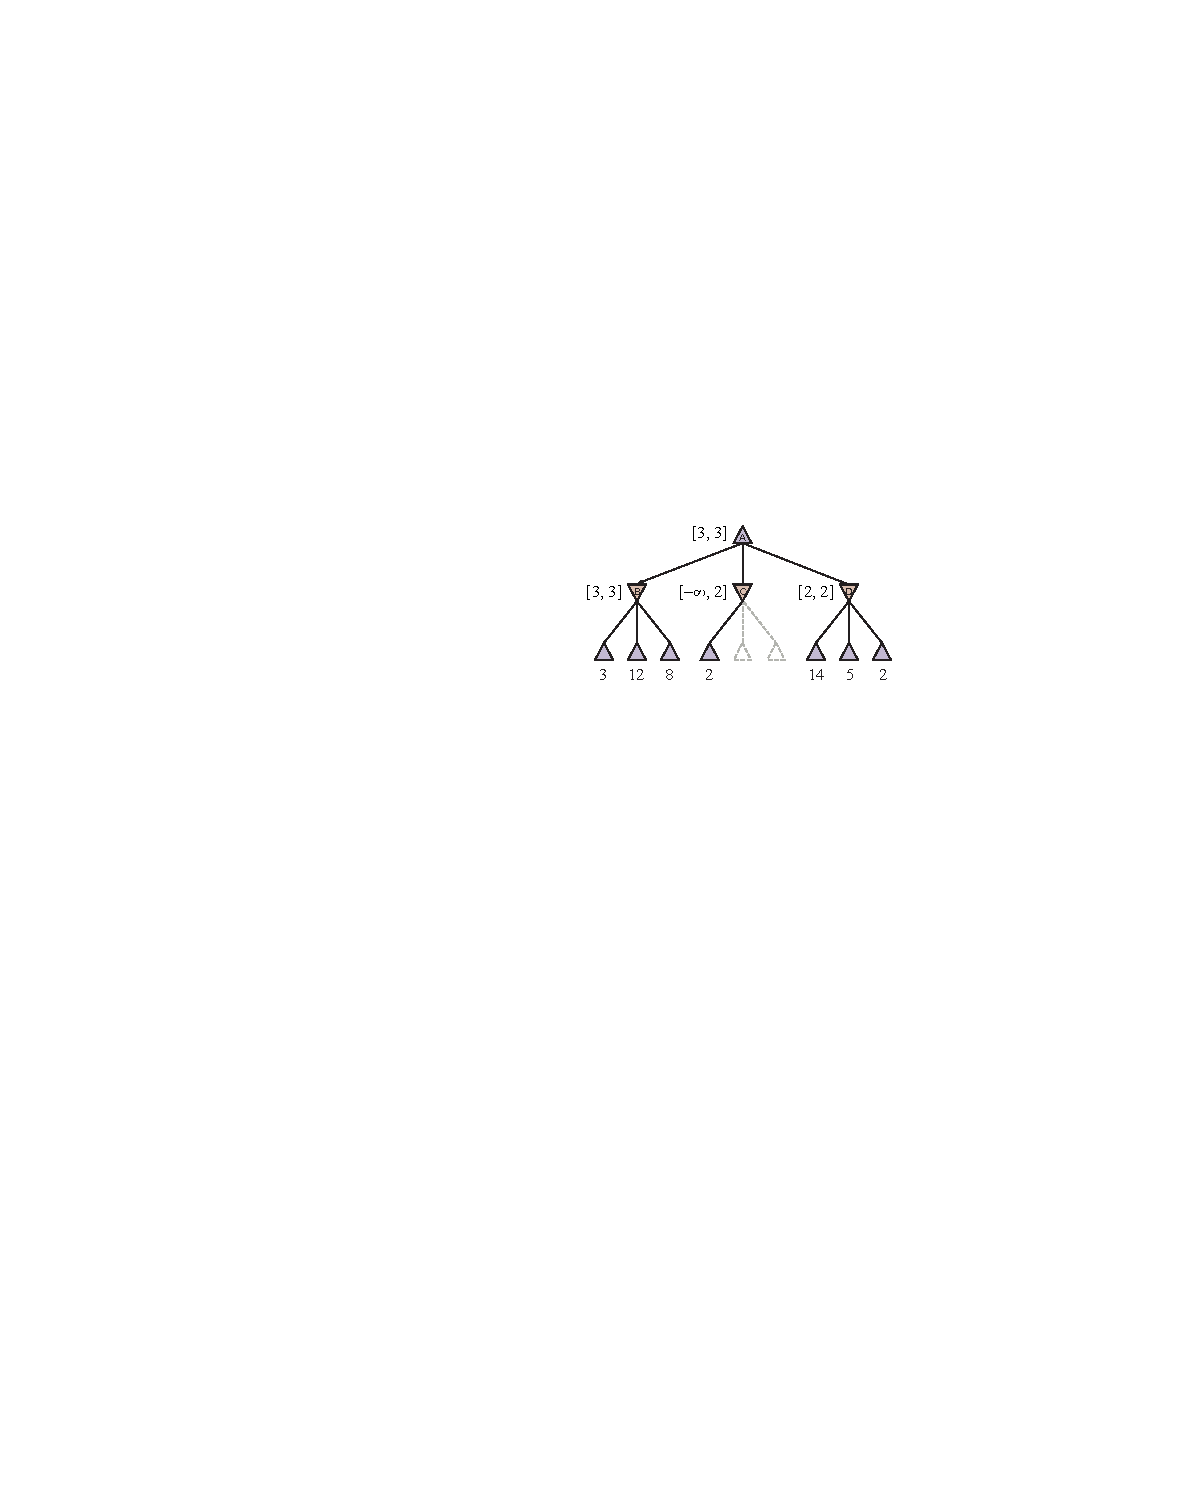
\includegraphics[alt={aima fig 05_05 f alpha beta tree},height=1.2in]{aima-fig-05_05-f-alpha-beta-tree.pdf}



\vspace{-.1in}
\begin{align*}
Minimax(root) &= max(min(3,12,8),min(2,x,y),min(14,5,2)) \\
              &= max(3,min(2,x,y),2) \\
              &= max(3,z,2) \text{ where } z = min(2,x,y) \le 2 \\
              &= 3.
\end{align*}
\vspace{-.2in}

In other words, the value of the root and hence the minimax decision are independent of the values of the leaves x and y, and therefore they can be pruned.
\section{Alpha-Beta Calculation Stages}
\label{sec:org3a98712}




\begin{itemize}
\item (a) 1st child of B has value 3. So B, a MIN node, has value \(\le\) 3.

\item (b) 2nd child of B has value 12; MIN would avoid, so B still \(\le\) 3.

\item (c) 3rd child of B has value 8; that's all B's children, so value of B exactly 3. Now infer value of root \(\ge\) 3 -- MAX picks max child value.

\item (d) 1st child of C has value 2. So C, a MIN node, value \(\le\) 2. But B is worth 3, so MAX won't choose C. No point looking at other children of C. \textbf{This is alpha–beta pruning}.

\item (e) 1st child of D value 14, so D worth \(\le\) 14. 14 still > 3, so need to keep exploring D's children. Now also back up 14 to root, which is new "at most", or \(\beta\), of root.

\item (f) 2nd child of D worth 5, so need to keep exploring for a value < 3. 3rd child is worth 2, so now D is worth exactly 2. So MAX's move is to B, giving a value of 3.
\end{itemize}





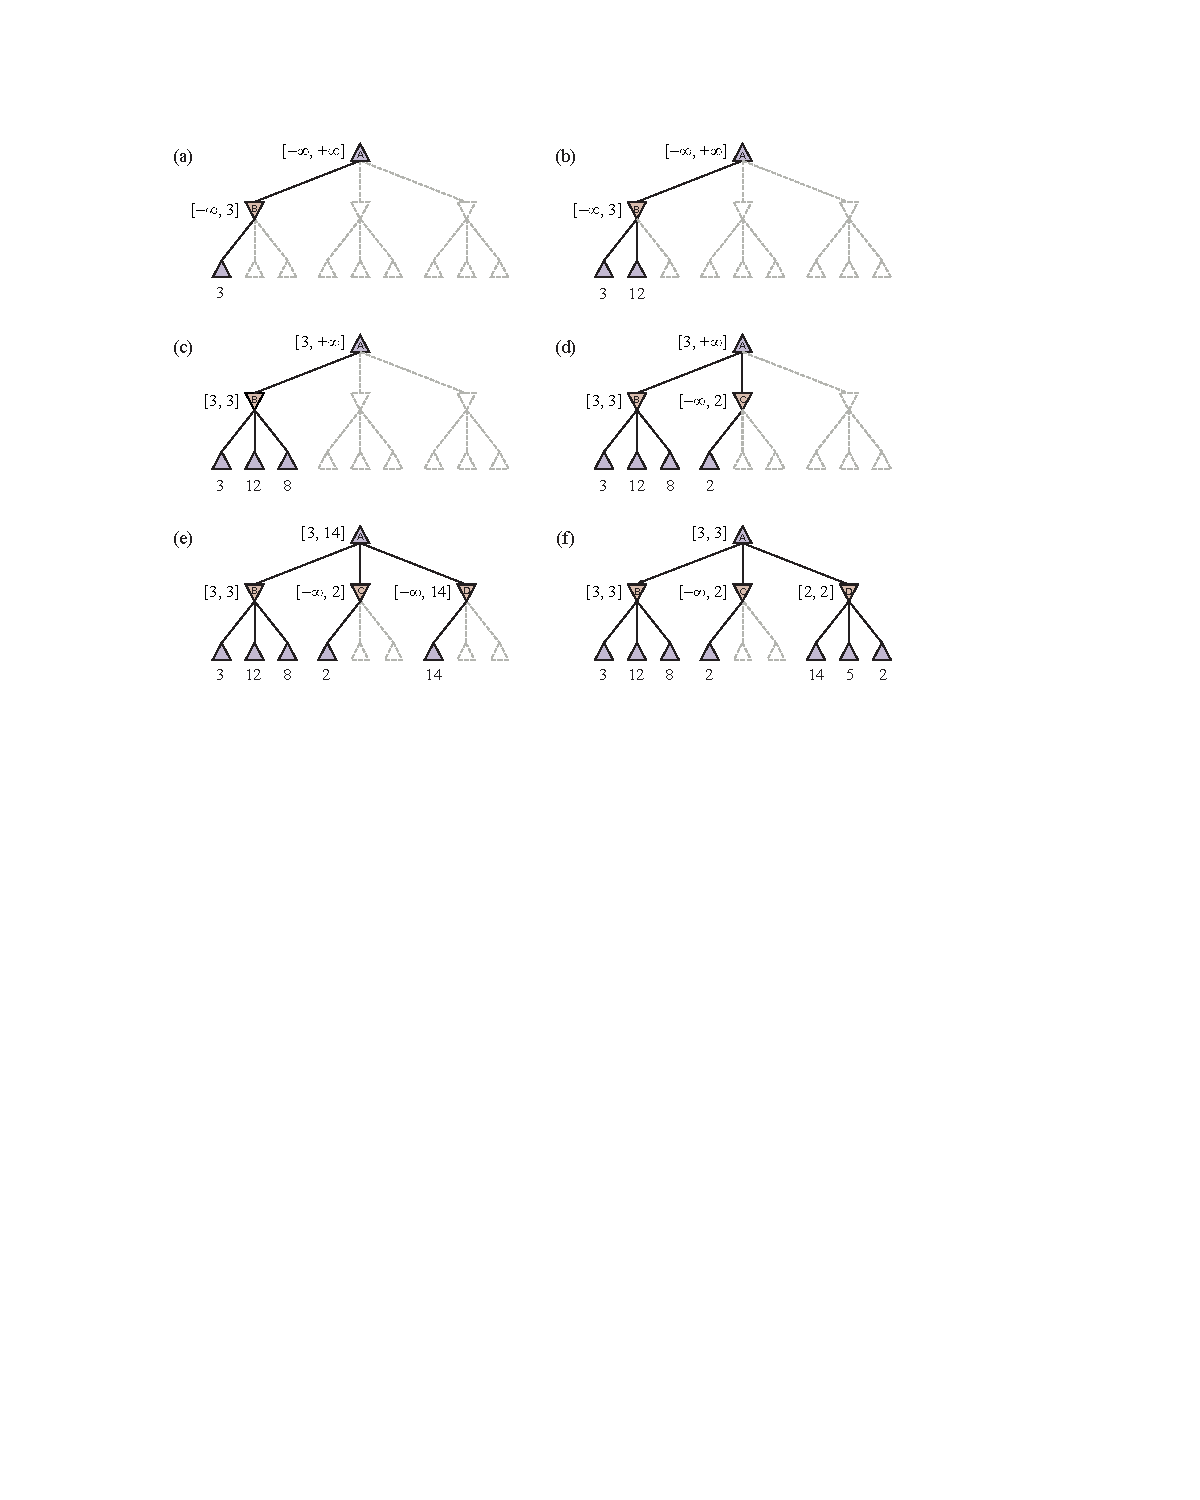
\includegraphics[alt={aima fig 05_05 game tree calculation stages},width=0.75\linewidth]{aima-fig-05_05-game-tree-calculation-stages.pdf}
\section{Alpha-Beta Search Algorithm}
\label{sec:orgbcec32e}




\begin{itemize}
\item Updates the values of \(\alpha\) and \(\beta\) as it goes along
\item Prunes the remaining branches at a node (i.e., terminates the recursive call) as soon as the value of the current node is known to be worse than the current \(\alpha\) for MAX, or \(\beta\) for MIN.
\end{itemize}






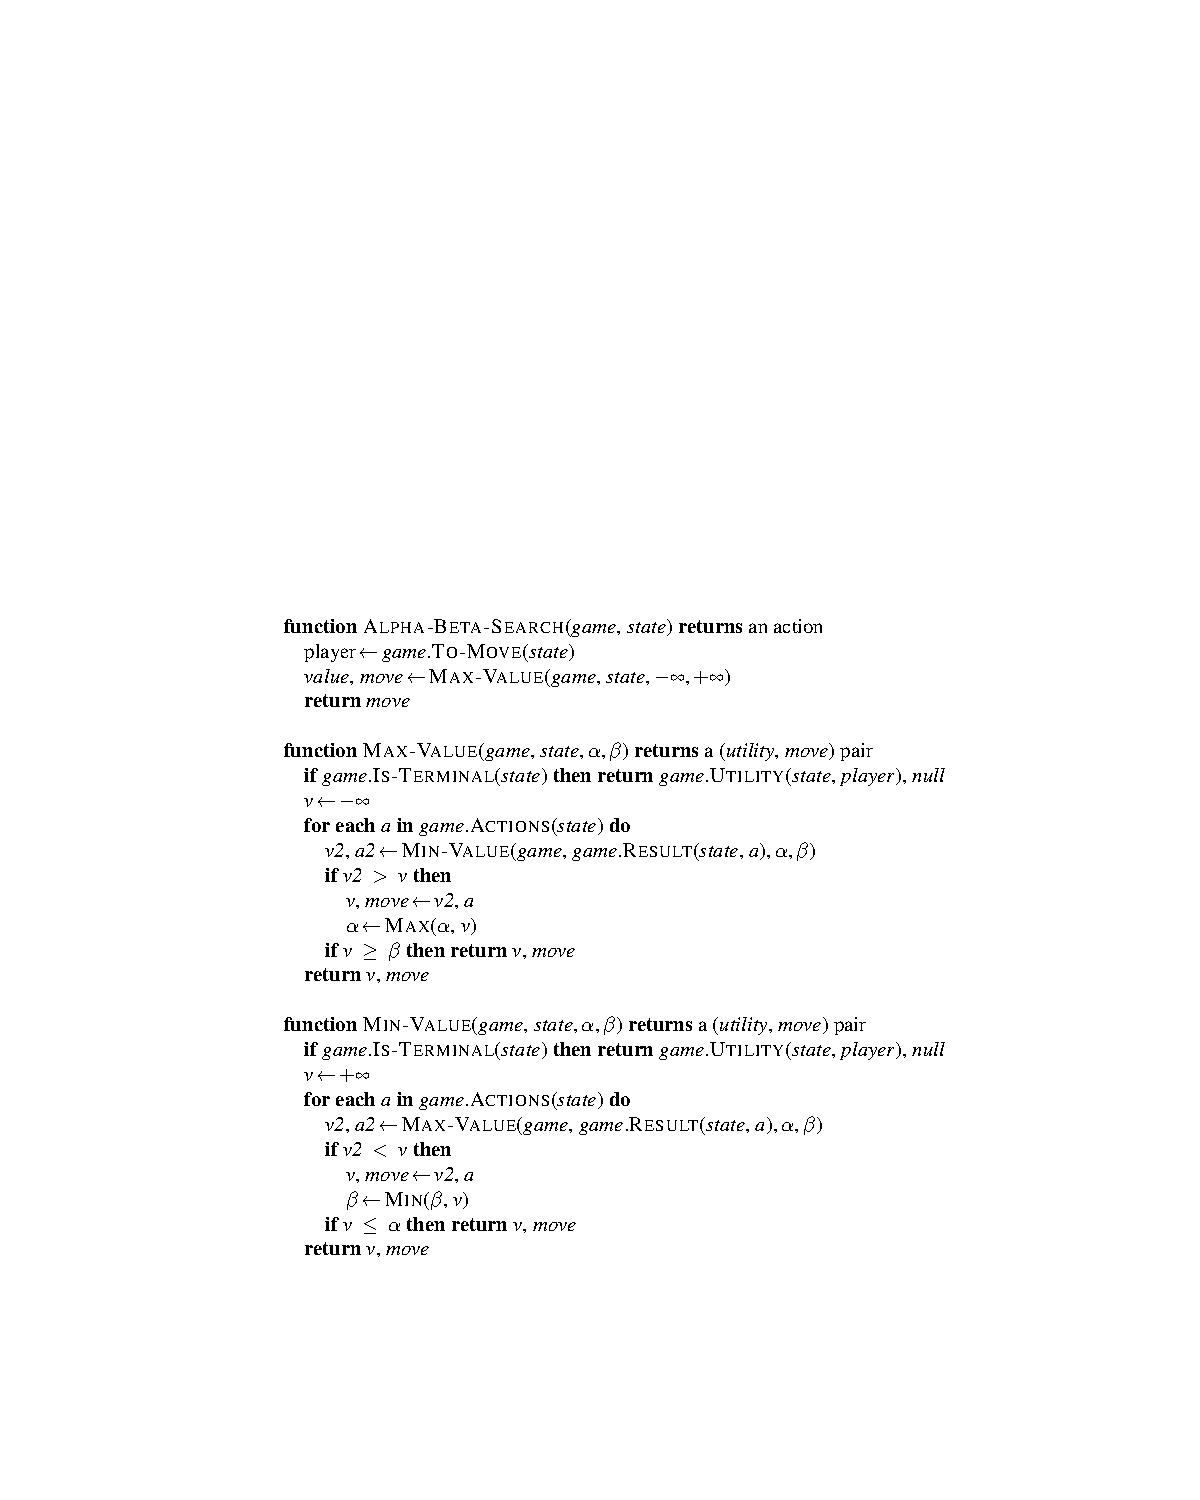
\includegraphics[alt={aima fig 05_07 alpha beta algorithm},width=0.75\linewidth]{aima-fig-05_07-alpha-beta-algorithm.pdf}
\section{Heuristic Alpha-Beta Tree Search}
\label{sec:org7097a8b}

Alpha-beta search helps, but it is still highly dependent on move ordering.  So we need more help in limiting search.

\begin{itemize}
\item We define a \textbf{heuristic evaluation function} that evaluates a static position.
\item We replace the terminal test with a cutoff test and use the heuristic evaluation function to determine the node's value.
\end{itemize}

\begin{equation*}
HMinimax(s, d) =
\begin{cases}
Eval(s,MAX)                                        & \text{if } IsCutoff(s, d) \\
max_{a \in Actions(s)} HMinimax(Result(s,a), d+1) & \text{if } ToMove(s) = MAX \\
min_{a \in Actions(s)} HMinimax(Result(s,a), d+1) & \text{if } ToMove(s) = MIN
\end{cases}
\end{equation*}
\section{Static Evaluation Functions}
\label{sec:orgac7cd4a}

A heuristic evaluation function \(Eval(s,p)\) returns an estimate of the expected utility of state \(s\) to player \(p\), just as the heuristic functions of Chapter 3 return an estimate of the distance to the goal.

\begin{itemize}
\item For terminal states, \(Eval(s,p) = Utility(s,p)\).
\item For nonterminal states, the evaluation must be somewhere between a loss and a win: \(Utility(loss,p) \le Eval(s,p)  \le Utility(win,p)\).
\end{itemize}

A popular form of hueristic evaluation function is a weighted linear evaluation function:

\begin{equation*}
Eval(s) = w_1 f_1(s) + w_2 f_2(s) + \cdots + w_n f_n(s) = \sum _{i=1}^n w_i f_i(s),
\end{equation*}

\begin{itemize}
\item Each \(f_i\) is a feature of the position such as "number of white bishops."
\item Each \(w_i\) is a weight saying how important that feature is.
\end{itemize}
\section{Chess Configuration Examples}
\label{sec:orgb2e40d4}


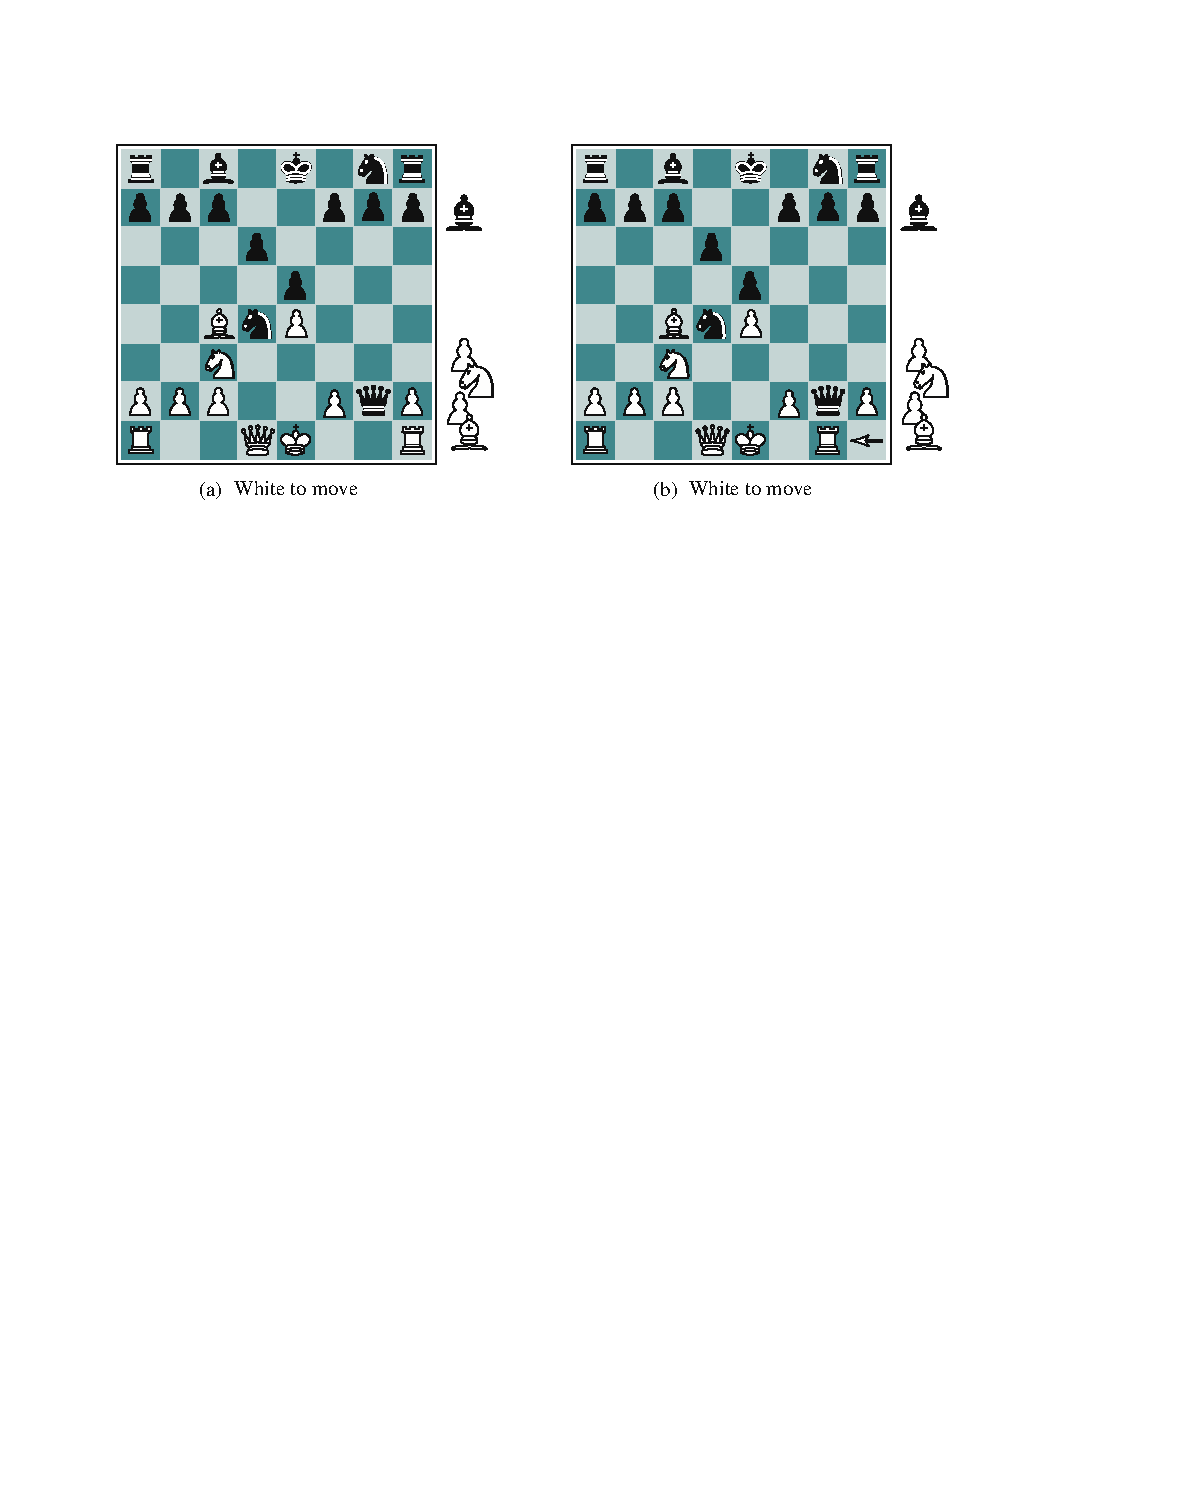
\includegraphics[alt={aima fig 05_08 chess positions},width=0.75\linewidth]{aima-fig-05_08-chess-positions.pdf}



\begin{itemize}
\item (a) Black has an advantage of a knight and two pawns, which should be enough to win the game.
\item (b) White will capture the queen, giving it an advantage that should be strong enough to win.
\end{itemize}
\section{Cutting Off Search}
\label{sec:org7094e78}

In alpha-beta search algorithm, keep track of depth so you can cut off at a particular depth and replace lines with \(IsTerminal(state)\) with

\begin{equation*}
\textbf{if } game.IsCutoff(state, depth) \textbf{ then return } game.Eval(state, player), null
\end{equation*}

Best to apply cutoff quiescent positions, that is, positions that don't contain a killer move that would radically change the value of the position.  Adding this to the \(IsCutoff\) function is called \textbf{quiescence search}.
\section{Horizon Effect}
\label{sec:org221ba0c}



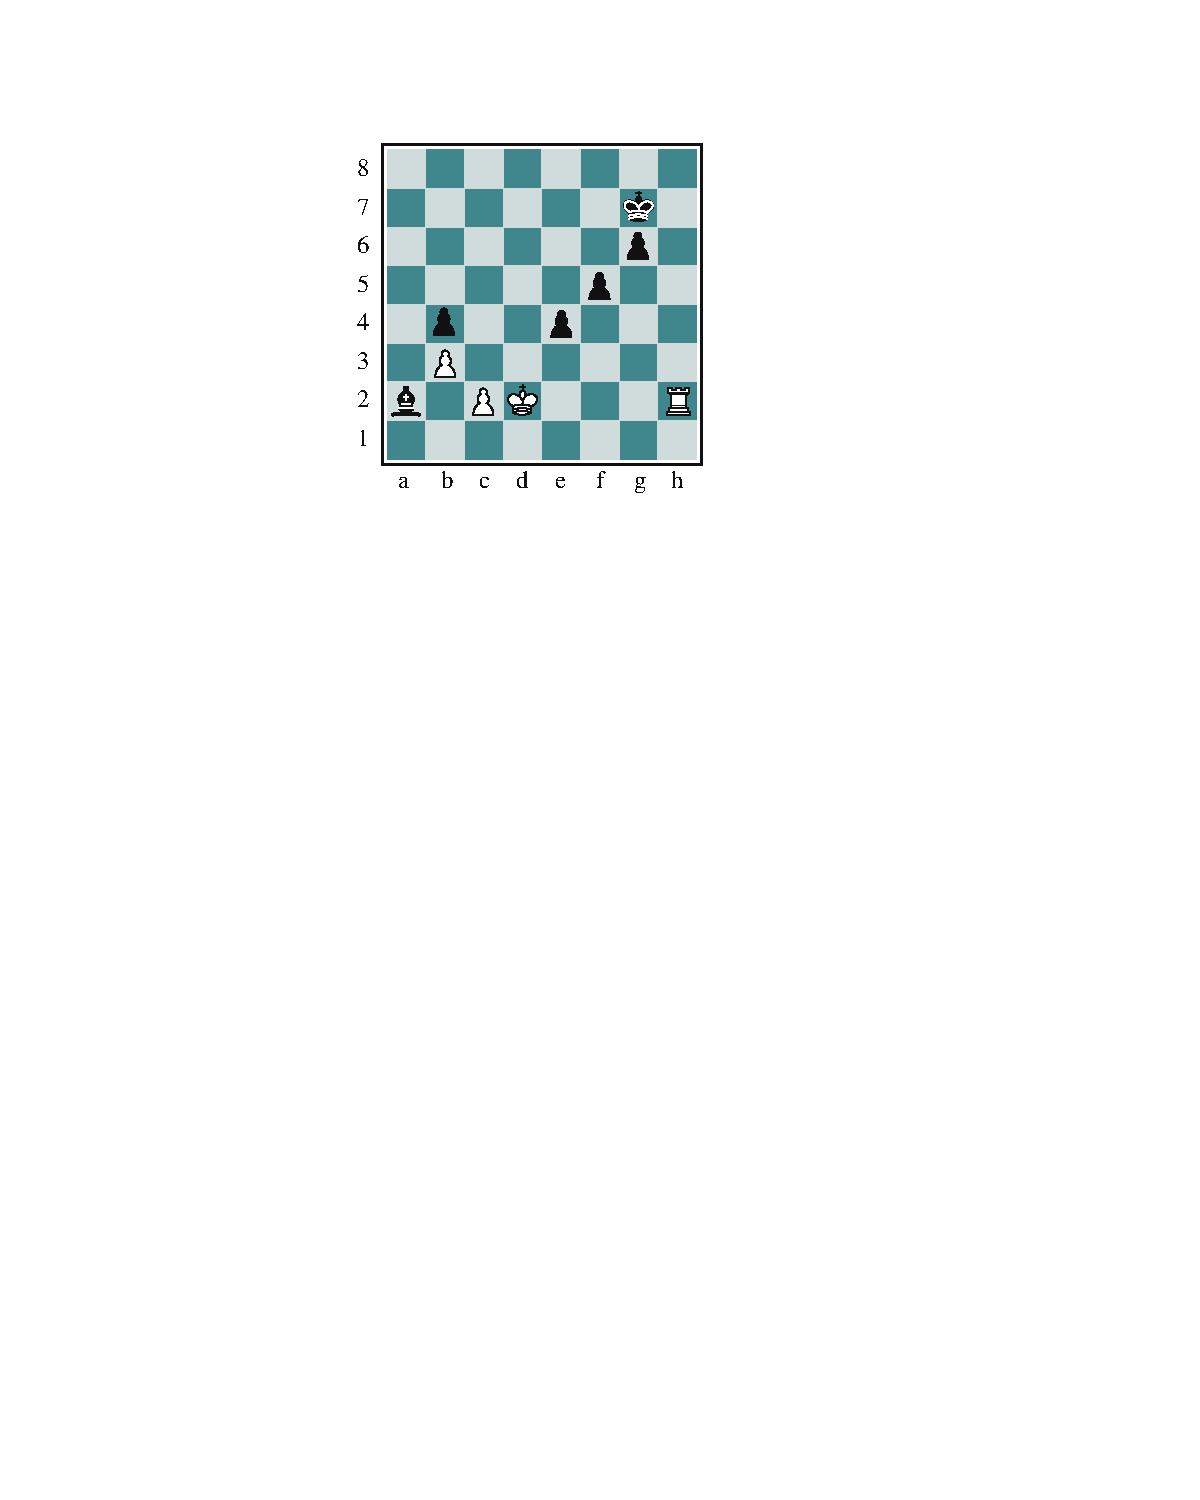
\includegraphics[alt={aima fig 05_09 chess horizon effect},height=2.0in]{aima-fig-05_09-chess-horizon-effect.pdf}



With Black to play, if Black only searches to a depth of 4-ply, it will see that

\begin{itemize}
\item moving the bishop either leads to its capture on b3, or to attack by the white rook moving to h1, but
\item playing \ldots{} e3+; Kxe3, f4+; Kxf4 sacrifices two pawns but "saves" the bishop.
\end{itemize}

This is an example of the horizon effect -- failing to see that these moves do not, in fact, save the bishop and ultimately result in a worse posiotion for black.
\section{Monte Carlo Tree Search (MCTS)}
\label{sec:org307e9f1}

Two major weaknesses of heuristic alpha-beta tree search:

\begin{itemize}
\item Can't handle high branching factors. Go has a branching factor that starts at 361, which means alpha–beta search would be limited to only 4 or 5 ply.

\item Can't always define a good static evaluation function.  E.g., in Go material value is not a strong indicator and most positions are in flux until the endgame.
\end{itemize}

MCTS:

Instead of searching to a given depth and applying a heurstic evaluation function to the resulting positions, we

\begin{itemize}
\item simulate complete games (from a given position) to terminal positions, and
\item back-up the win/loss scores up the tree.
\end{itemize}

Playout policy: bias move selection towards good ones.  Two options:

\begin{itemize}
\item Pure MCTS: do \(N\) simulations, track which move leads to highest win percentage.
\item Selection policy: focus computation on important parts of game tree by balancing exploration and exploitation.
\end{itemize}
\section{Selection-Based MCTS Algorithm}
\label{sec:org396aadd}


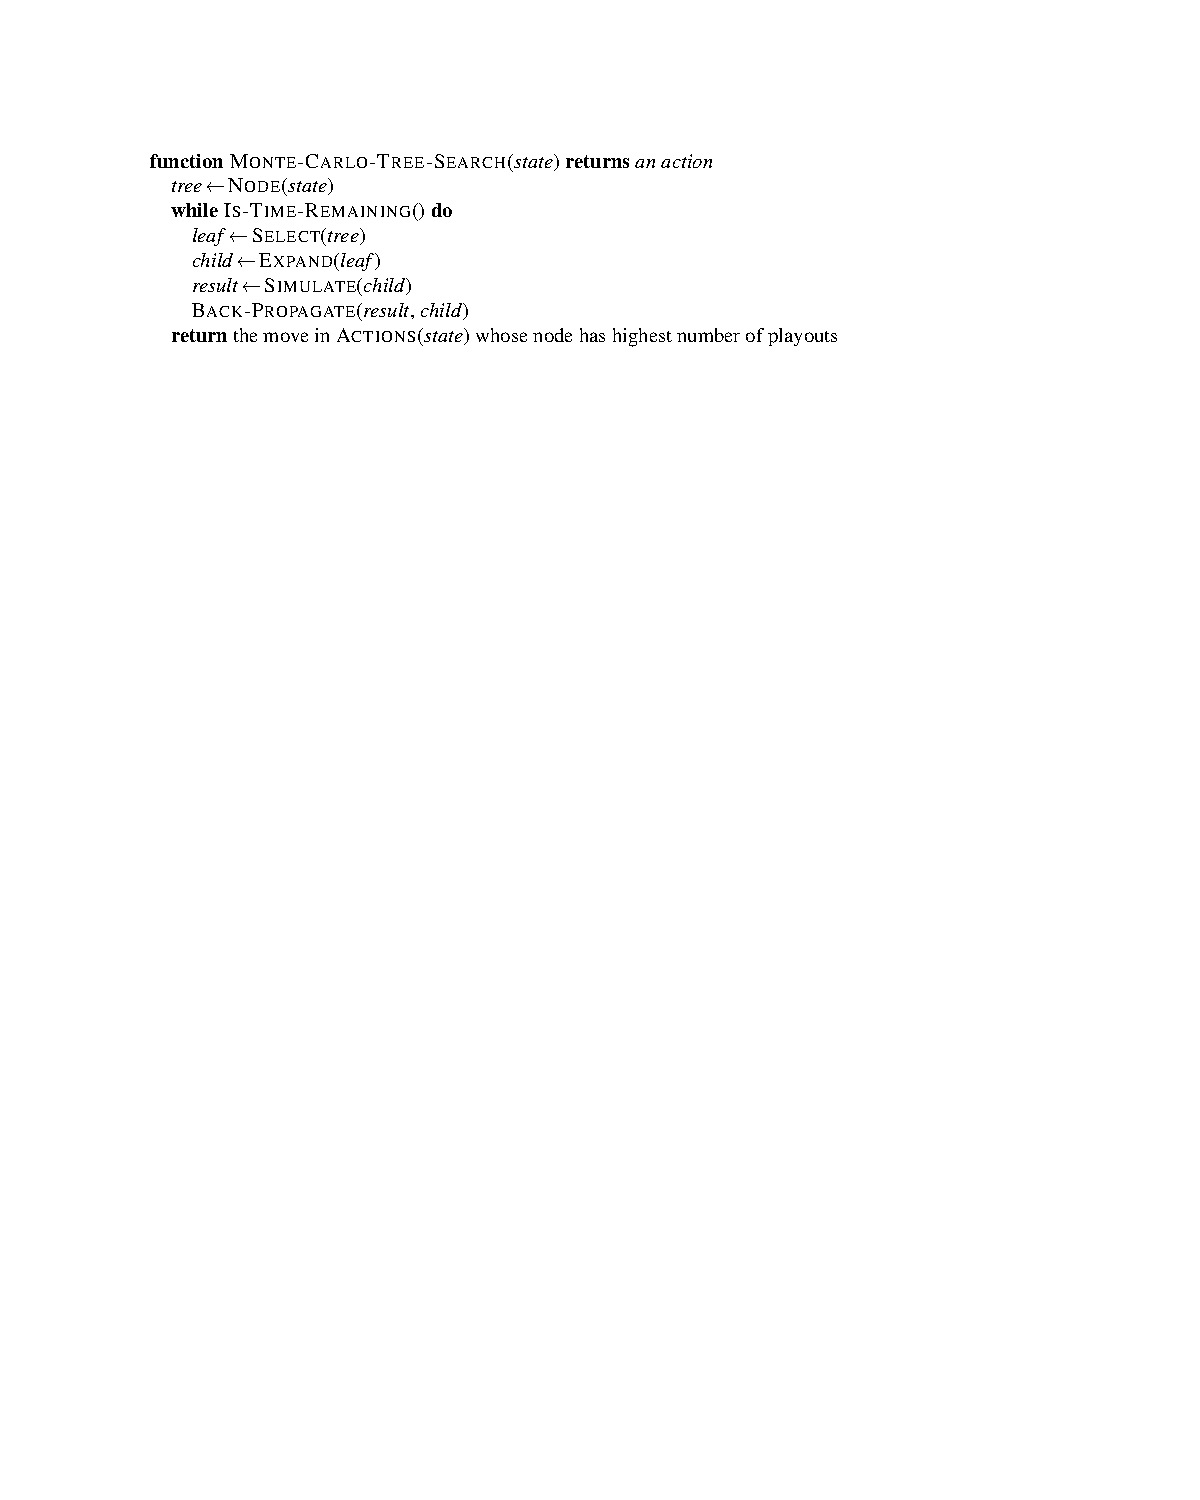
\includegraphics[alt={aima fig 05_11 mcts algorithm},height=1.6in]{aima-fig-05_11-mcts-algorithm.pdf}



\begin{itemize}
\item Selection: starting at root, choose a move leading to a successor node, and repeat that process, moving down the tree to a leaf.

\item Expansion: grow the search tree by generating a new child of the selected node.

\item Simulation: perform a playout from the newly generated child node, choosing moves for both players according to the playout policy. These moves are not recorded in the search tree. In the next slide, the simulation results in a win for black.

\item Back-propagation: use the result of the simulation to update all search tree nodes going up to the root.
\end{itemize}
\section{MCTS Iteration}
\label{sec:org3df325e}

White just played (light purple nodes) -- black to play.


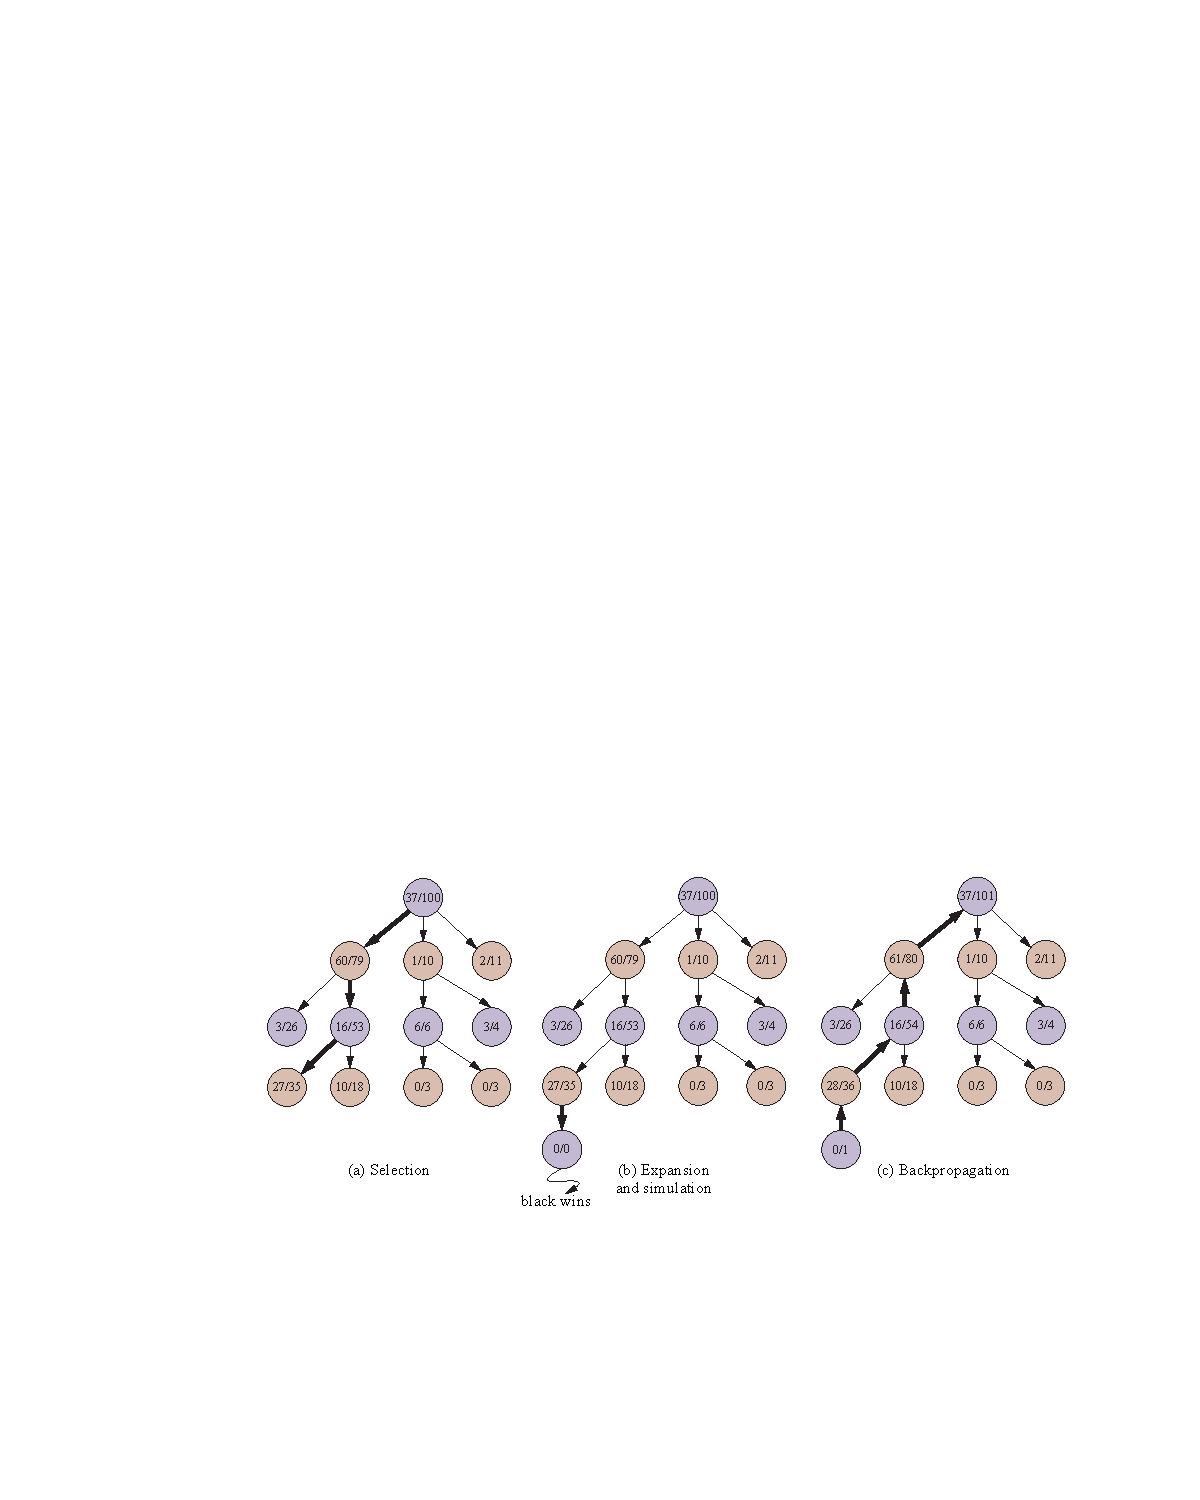
\includegraphics[alt={aima fig 05_10 mcts iteration},height=1.6in]{aima-fig-05_10-mcts-iteration.pdf}



\begin{itemize}
\item (a) Select moves, all the way down the tree, ending at the leaf node marked 27/35 (27 wins for black out of 35 playouts).
\item (b) Expand the selected node and do a simulation (playout), which ends in a win for black.
\item (c) The results of the simulation are back-propagated up the tree.

\begin{itemize}
\item Since black won the playout, black nodes are incremented in both number of wins and number of playouts, so 27/35 \(\rightarrow\) 28/36,  60/79 \(\rightarrow\) 61/80.
\item White lost, so white nodes incremented in number of playouts, so 16/53 \(\rightarrow\) 16/54, root 37/100 \(\rightarrow\)  37/101.
\end{itemize}
\end{itemize}
\section{Upper Confidence Bound MCTS Selection Policy}
\label{sec:org7df2a45}

\begin{equation*}
UCB1(n) = \overbrace{\frac{U(n)}{N(n)}}^{\text{Exploitation Term}} + C \times \overbrace{\sqrt{ \frac{\log N (PARENT(n))}{N(n)} }}^{\text{Exploration Term}}
\end{equation*}


\begin{itemize}
\item \(U(n)\): total utility of all playouts that went through node \(n\),
\item \(N(n)\): number of playouts through node \(n\), \(PARENT(n)\) is parent node of \(n\) in tree,
\item \(C\): constant that balances exploitation and exploration.

\begin{itemize}
\item Theoretically, \(C = \sqrt{2}\) is best.
\item In practice, programmers try different values.
\item AlphaZero adds move probability term, calculated by neural network trained on past self-play.
\end{itemize}
\end{itemize}


Remember that MCTS returns the node with the highest number of playouts, not the node with the highest average utility.  Why?

\begin{itemize}
\item A node with 65/100 wins better than one with 2/3 wins, due to lower uncertainty.
\item UCB1 ensures that node with most playouts is almost always node with highest win percentage -- selection process increasingly favors win percentage as number of playouts increases.
\end{itemize}
\section{UCB1 In Action -- Exploitation}
\label{sec:org904fa65}





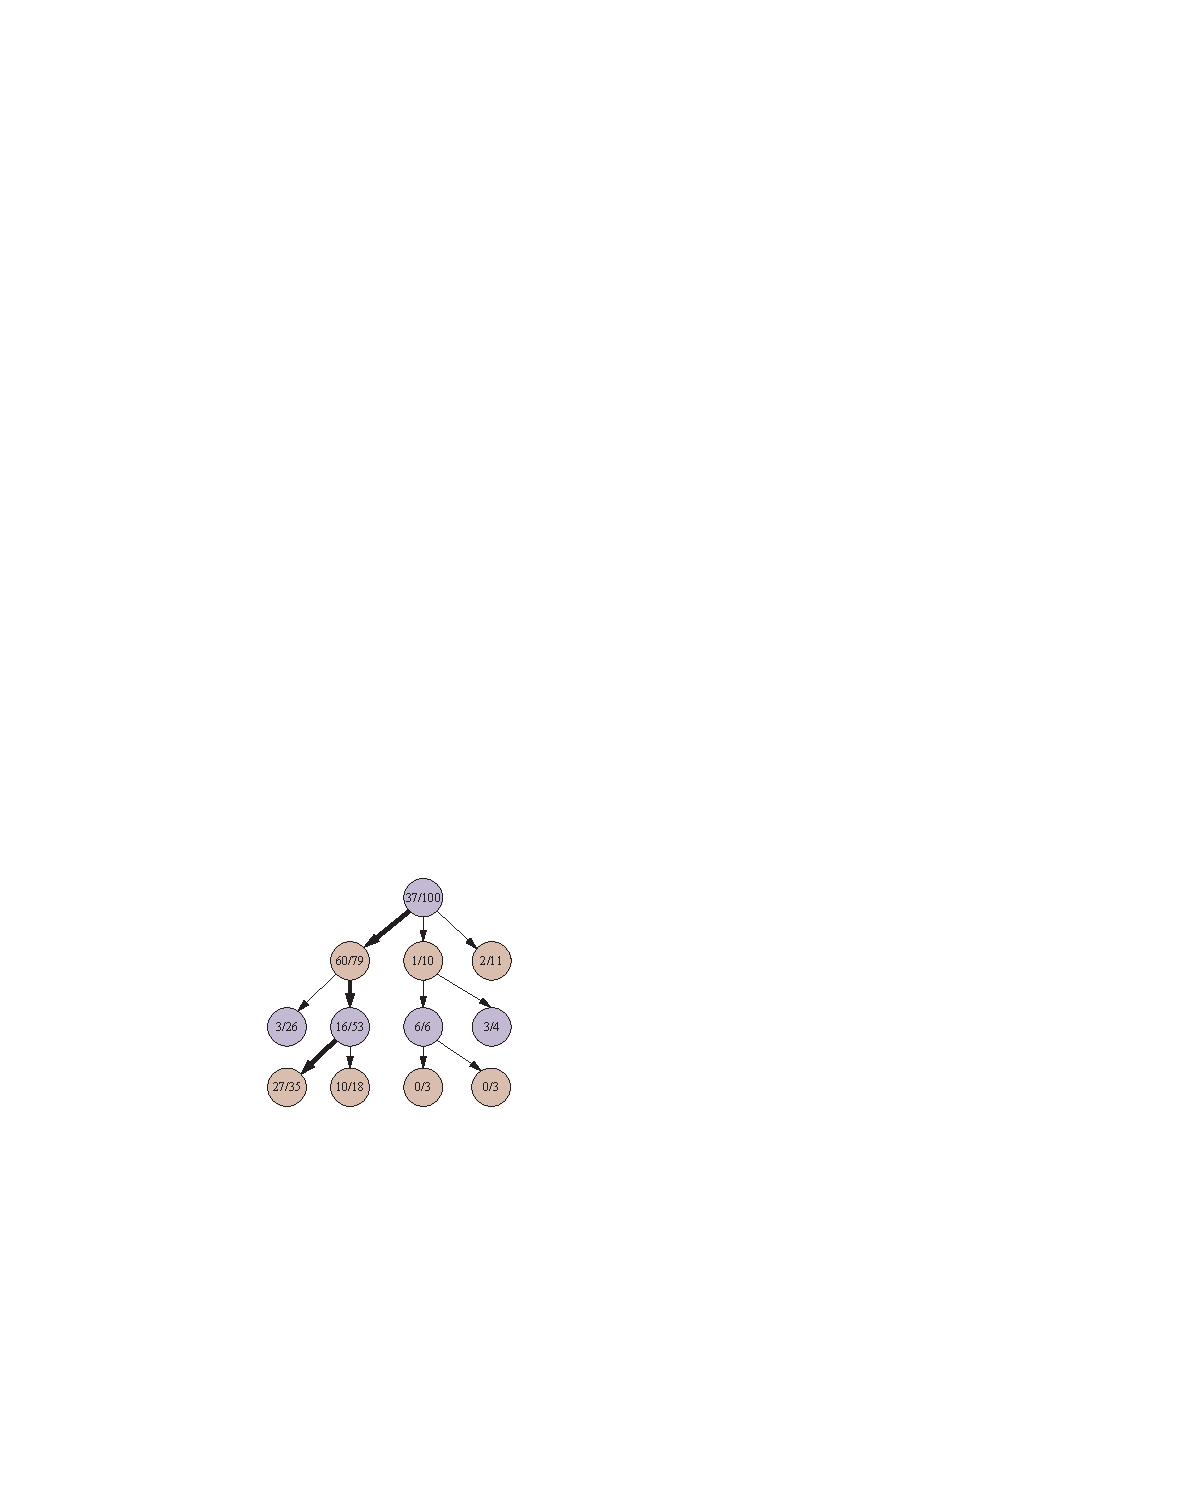
\includegraphics[alt={aima fig 05_10 a mcts selection},width=0.75\linewidth]{aima-fig-05_10-a-mcts-selection.pdf}






With \(C = 1.4\),

\begin{itemize}
\item the 60/79 node:
\end{itemize}

\begin{align*}
UCB1(n) &= \frac{U(n)}{N(n)} + C \times \sqrt{ \frac{\log N (PARENT(n))}{N(n)} }\\
        &= \frac{60}{79} + 1.4 \times \sqrt{ \frac{\log 100}{79} }\\
        &= 1.1 \checkmark
\end{align*}

\begin{itemize}
\item and the 2/11 node:
\end{itemize}

\begin{align*}
UCB1(n) &= \frac{U(n)}{N(n)} + C \times \sqrt{ \frac{\log N (PARENT(n))}{N(n)} }\\
        &= \frac{2}{11} + 1.4 \times \sqrt{ \frac{\log 100}{11} }\\
        &= 1.09
\end{align*}
\section{UCB1 In Action -- Exploration}
\label{sec:orgd8094eb}





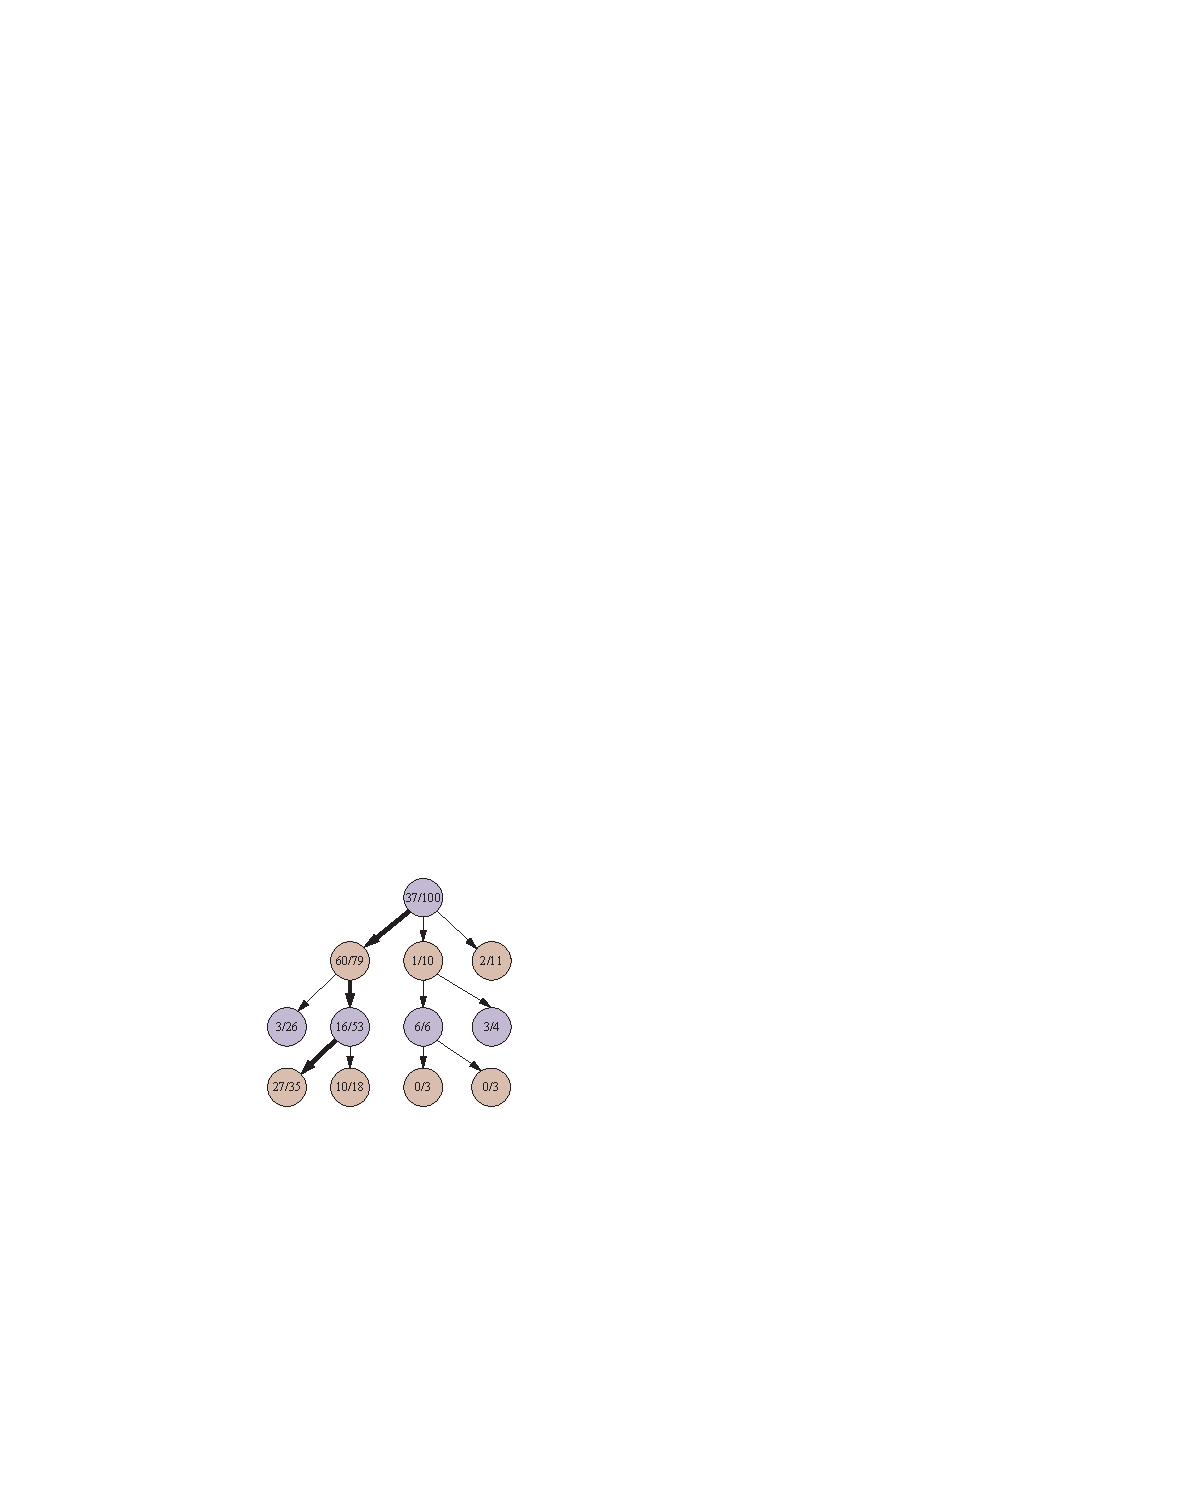
\includegraphics[alt={aima fig 05_10 a mcts selection},width=0.75\linewidth]{aima-fig-05_10-a-mcts-selection.pdf}






With \(C = 1.5\),

\begin{itemize}
\item the 60/79 node
\end{itemize}

\begin{align*}
UCB1(n) &= \frac{U(n)}{N(n)} + C \times \sqrt{ \frac{\log N (PARENT(n))}{N(n)} }\\
        &= \frac{60}{79} + 1.5 \times \sqrt{ \frac{\log 100}{79} }\\
        &= 1.12
\end{align*}

\begin{itemize}
\item and the 2/11 node:
\end{itemize}

\begin{align*}
UCB1(n) &= \frac{U(n)}{N(n)} + C \times \sqrt{ \frac{\log N (PARENT(n))}{N(n)} }\\
        &= \frac{2}{11} + 1.5 \times \sqrt{ \frac{\log 100}{11} }\\
        &= 1.15 \checkmark
\end{align*}
\section{Errors in Heuristic Minimax Search}
\label{sec:org584844a}


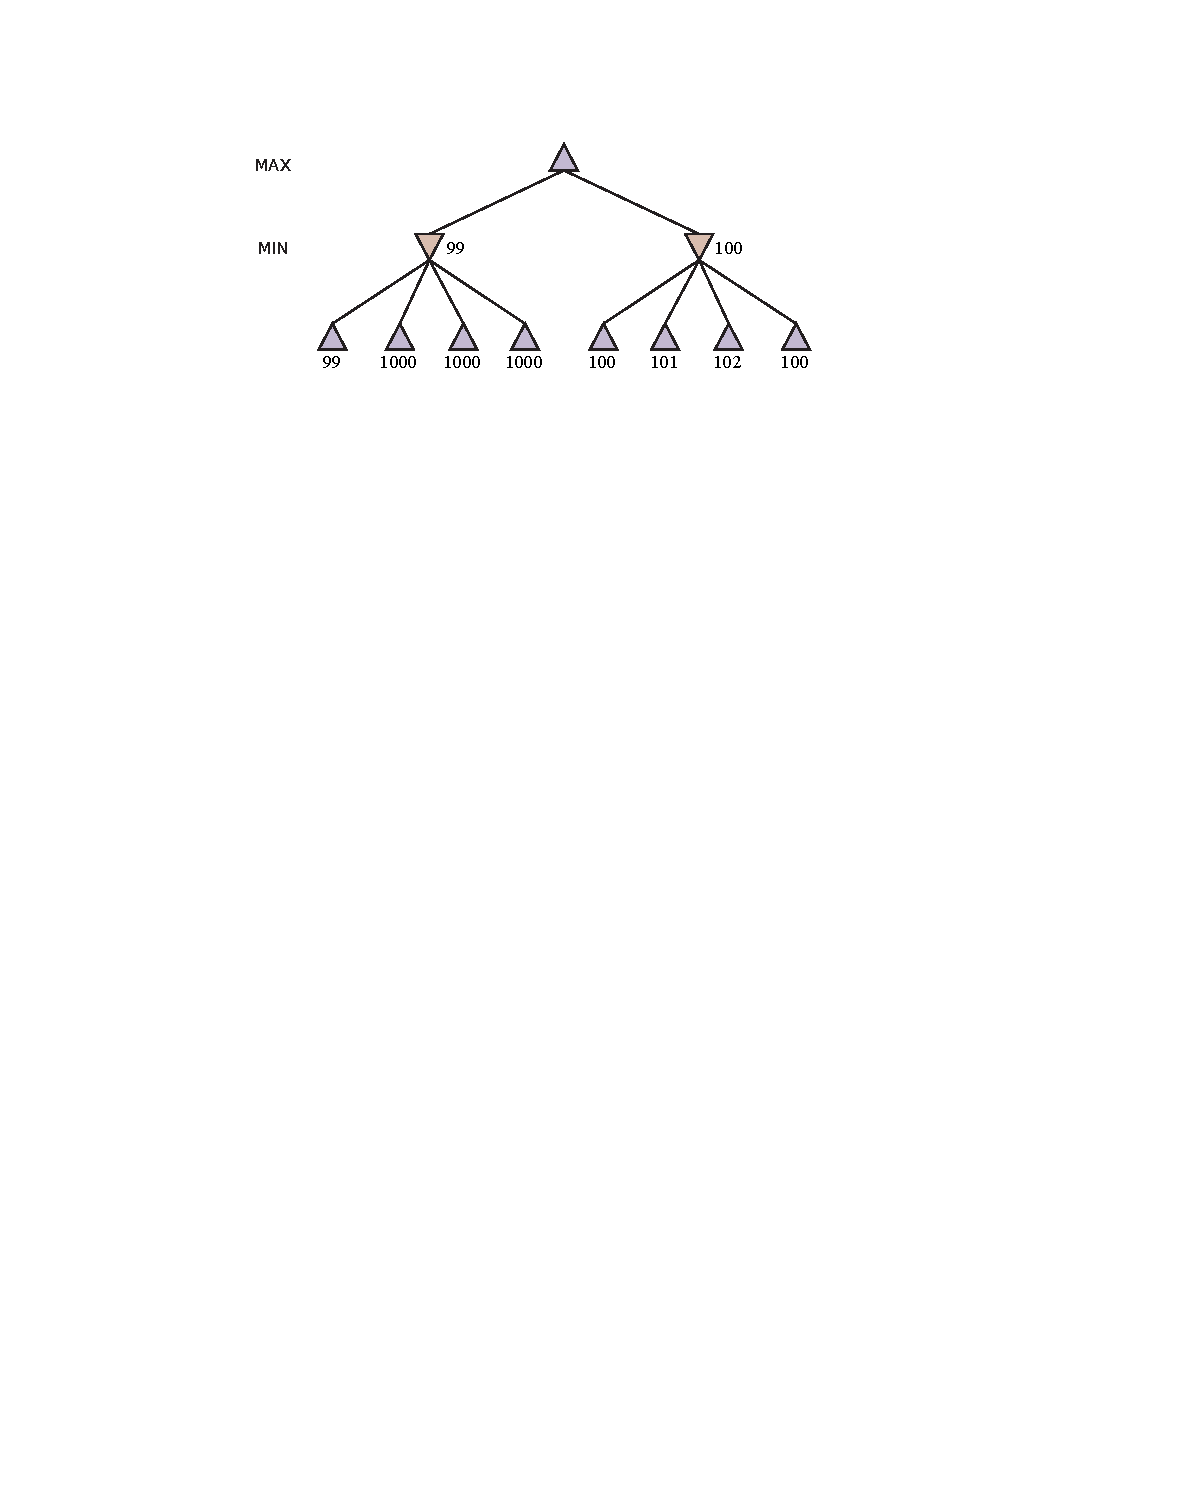
\includegraphics[alt={aima fig 05_16 heuristic minimax errors},width=0.75\linewidth]{aima-fig-05_16-heuristic-minimax-errors.pdf}



\begin{itemize}
\item If evaluation function is 100\% correct, right branch is correct.
\item If evaluation function has random error with \(\sigma = 5\), left is better 71\% of the time because one of the four right-hand leaves will dip below 99.
\item If evaluation function has random error with \(\sigma = 2\), left is better 58\% of the time.
\end{itemize}
\section{Closing Thoughts}
\label{sec:orga3a1f5c}

The game playing algorithms we considered here have limitations that we will address in furture lessons.

\begin{itemize}
\item Vulnerability to errors in the heuristic function. (See Previous slide.)
\item Sometimes there is a single clearly best move, but Alpha-beta and MCTS waste computation by calculating values of many legal moves.

\begin{itemize}
\item Better to employ metareasoning about the utility of node expansion -- only expand nodes likely to lead to a better move.
\end{itemize}

\item Alpha-beta and MCTS reason about individual moves.  Humans reason abstractly, selectively forming plausible plans to acheive (intermediate) goals, e.g., trapping the opponent's queen.

\begin{itemize}
\item We will learn about such approaches when we study \textbf{planning}.
\end{itemize}

\item Alpha-beta (and MCTS when depth-limited) rely on human-crafted evaluation functions.

\begin{itemize}
\item Programs like AlphaZero[\textsuperscript{AlphaZero}] need only the rules of the game to learn how to play at superhuman levels.
\end{itemize}
\end{itemize}


{[}\textsuperscript{AlphaZero}]: \url{https://arxiv.org/pdf/1712.01815}
\end{document}
